\documentclass[journal,10pt,twocolumn]{article}
\usepackage{graphicx}
\usepackage[margin=0.5in]{geometry}
\usepackage{amsmath}
\usepackage{kvmap}
\title{\textbf{AVR-GCC Assignment}}
\author{Mohamed Hamdan}
\date{August 2022}

\begin{document}
\maketitle
\paragraph{\textit{Problem Statement} - A sequential circuit has a single input x and a single output z. The input signal x can occur in groups of 1, 2 and 3 pulses. If x = 1 for one clock period, the output z will be 1 for three clock periods before returning to the starting state. If x = 1 for two clock periods, the output z will be 1 for two clock periods before returning to the starting state. If x = 1 for three clock periods, the output z will be 1 for a single clock period before returning to the starting state. Construct a state diagram and implement your design with D F F s . The circuit when designed acts as a pulse width adjuster.
}

\section*{\large Hardware}
\subsection*{\normalsize Components}
{
\centering
\begin{tabular}{|c|c|c|}
\hline
Component&Value&Count\\
\hline
Arduino&uno&1\\
\hline
Flip Flop&7474&2\\
\hline
LED&Red&1\\
\hline
Resistor&220ohm&1\\
\hline
Jumper wires&-&as required\\
\hline
\end{tabular}\par
}
\subsection*{\normalsize Connections}
The following connections are to be read as \textbf{IC-Name-IC-pin no:Arduino-pin no} :
\begin{itemize}
\item \textbf{IC7447(1)} - (1:5.5V), (2:8), (3:13), (4:5.5V), (5:2), (6:None), (7:Gnd), (8:None), (9:3), (10:5.5V), (11:13), (12:9), (13:5.5V), (14:5.5V)
\item \textbf{IC7447(2)} - (1:5.5V), (2:10), (3:13), (4:5.5V), (5:4), (6:None), (7:Gnd), (8:None), (9:5), (10:5.5V), (11:13), (12:11), (13:5.5V), 
 (14:5.5V)
\end{itemize}
Connect LED to pin 12 of arduino with the 220ohm resistor in series. Use pin 6 of arduino to input X.

\section*{\large State Diagram}
The state diagram shown in \ref{fig:state_diagram} can be understood easily by grouping the states according to the clock pulse number. Consider one cycle of the state machine to contain three clock pulses numbered 1, 2 and 3. The states 0, 1 and 2 in the clock-1 group are the entry states to produce the Z values for the successive 2 clock pulses (clock-2 and clock-3). Distinct entry states are necessary in order to remember the input sequence of the previous cycle. While entering into any of these three states, the Z value for clock-1 is already determined by the input at clock-3 of the previous cycle. In order to keep track of the number of ones in the input sequence X and to output the proper values at Z (determined by the entry state), the remaining 7 states (3-9) are required.\\
Since the state diagram uses 10 states, the design requires 4 DFFs. Let the present state be denoted by $\textbf{P} = P_3P_2P_1P_0$ and the next state as $\textbf{S} = S_3S_2S_1S_0$ with $X$ as input and $Z$ as output.
\begin{figure}[ht]
\centering
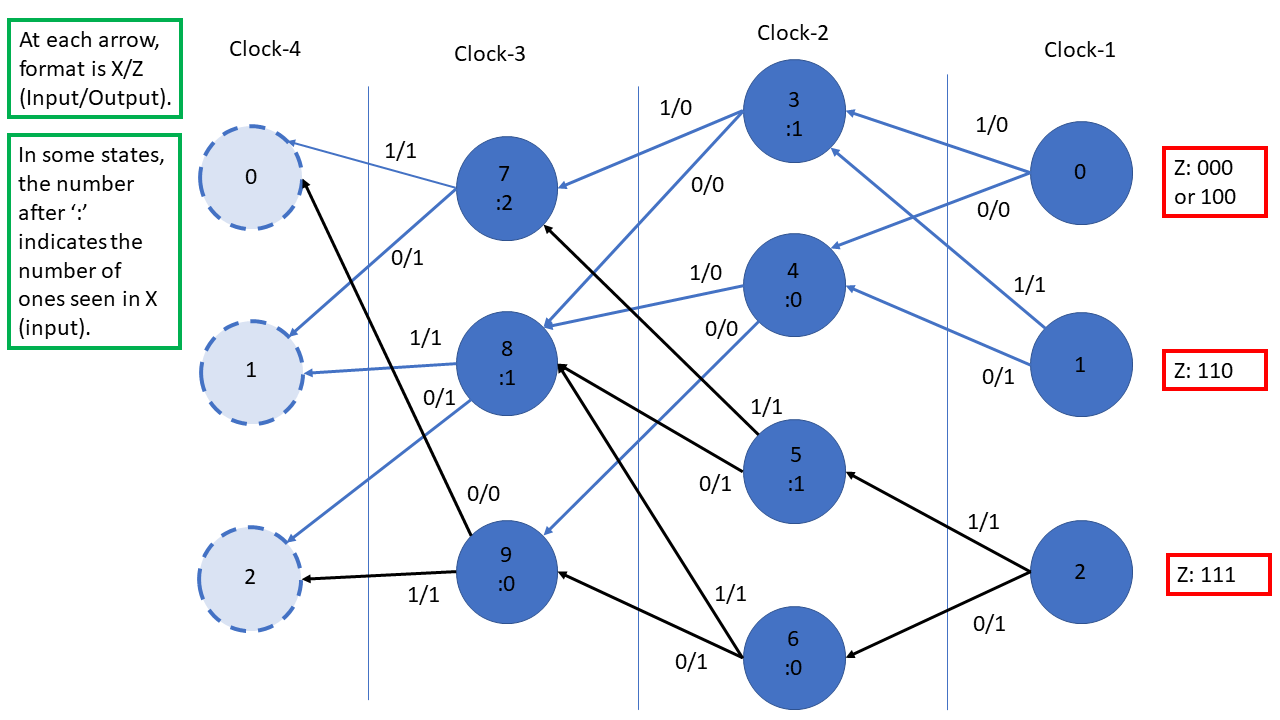
\includegraphics[width=1\columnwidth]{state_diagram.png}
\caption{State diagram for pulse width adjuster}
\label{fig:state_diagram}
\end{figure}
\section*{\large Truth table}
{
\centering
\begin{tabular}{|c|c|c|c|c|c|c|c|c|c|}
\hline
$\boldsymbol{P_3}$&$\boldsymbol{P_2}$&$\boldsymbol{P_1}$&$\boldsymbol{P_0}$&$\boldsymbol{X}$&$\boldsymbol{S_3}$&$\boldsymbol{S_2}$&$\boldsymbol{S_1}$&$\boldsymbol{S_0}$&$\boldsymbol{Z}$\\
\hline
0&0&0&0&0&0&1&0&0&0\\%
\hline
0&0&0&0&1&0&0&1&1&0\\%
\hline
0&0&0&1&0&0&1&0&0&1\\%
\hline
0&0&0&1&1&0&0&1&1&1\\%
\hline
0&0&1&0&0&0&1&1&0&1\\%
\hline
0&0&1&0&1&0&1&0&1&1\\%
\hline
0&0&1&1&0&1&0&0&0&0\\%
\hline
0&0&1&1&1&0&1&1&1&0\\%
\hline
0&1&0&0&0&1&0&0&1&0\\%
\hline
0&1&0&0&1&1&0&0&0&0\\%
\hline
0&1&0&1&0&1&0&0&0&1\\%
\hline
0&1&0&1&1&0&1&1&1&1\\%
\hline
0&1&1&0&0&1&0&0&1&1\\%
\hline
0&1&1&0&1&1&0&0&0&1\\%
\hline
0&1&1&1&0&0&0&0&1&1\\%
\hline
0&1&1&1&1&0&0&0&0&1\\%
\hline
1&0&0&0&0&0&0&1&0&1\\%
\hline
1&0&0&0&1&0&0&0&1&1\\%
\hline
1&0&0&1&0&0&0&0&0&0\\%
\hline
1&0&0&1&1&0&0&1&0&1\\%
\hline
1&0&1&0&0&X&X&X&X&X\\%
\hline
\end{tabular}\par
}
{
\centering
\begin{tabular}{|c|c|c|c|c|c|c|c|c|c|}
\hline
$\boldsymbol{P_3}$&$\boldsymbol{P_2}$&$\boldsymbol{P_1}$&$\boldsymbol{P_0}$&$\boldsymbol{X}$&$\boldsymbol{S_3}$&$\boldsymbol{S_2}$&$\boldsymbol{S_1}$&$\boldsymbol{S_0}$&$\boldsymbol{Z}$\\
\hline
1&0&1&0&1&X&X&X&X&X\\%
\hline
1&0&1&1&0&X&X&X&X&X\\%
\hline
1&0&1&1&1&X&X&X&X&X\\%
\hline
1&1&0&0&0&X&X&X&X&X\\%
\hline
1&1&0&0&1&X&X&X&X&X\\%
\hline
1&1&0&1&0&X&X&X&X&X\\%
\hline
1&1&0&1&1&X&X&X&X&X\\%
\hline
1&1&1&0&0&X&X&X&X&X\\%
\hline
1&1&1&0&1&X&X&X&X&X\\%
\hline
1&1&1&1&0&X&X&X&X&X\\%
\hline
1&1&1&1&1&X&X&X&X&X\\%
\hline
\end{tabular}\par
}

\section*{\large Minimization using Kmap} 
\begin{kvmap}
\kvlist{4}{8}{0,0,0,0,0,0,0,1,1,1,0,0,1,1,0,1,x,x,x,x,x,x,x,x,x,x,x,x,0,0,0,0}{P_0,X,P_3,P_2,P_1}
\bundle[color=red]{0}{2}{1}{6}
\bundle[invert=true,color=blue]{0}{3}{3}{4}
\bundle[color=green]{3}{1}{3}{1}
\bundle[color=green]{3}{6}{3}{6}
\end{kvmap}

\begin{kvmap}
\kvlist{4}{8}{1,0,0,1,1,1,1,0,0,0,0,0,0,0,1,0,x,x,x,x,x,x,x,x,x,x,x,x,0,0,0,0}{P_0,X,P_3,P_2,P_1}
\bundle[color=red]{0}{1}{1}{1}
\bundle[color=red]{0}{6}{1}{6}
\bundle[color=blue, reducespace=2pt]{1}{1}{2}{1}
\bundle[color=blue, reducespace=2pt]{1}{6}{2}{6}
\bundle[invert=true,color=green]{0}{0}{3}{0}
\bundle[color=black]{2}{3}{2}{4}
\end{kvmap}

\begin{kvmap}
\kvlist{4}{8}{0,1,1,0,1,0,1,0,0,0,0,0,0,0,1,0,x,x,x,x,x,x,x,x,x,x,x,x,1,0,1,0}{P_0,X,P_3,P_2,P_1}
\bundle[color=red]{2}{0}{2}{1}
\bundle[color=red]{2}{7}{2}{6}
\bundle[invert=true,color=blue,reducespace=2pt]{2}{0}{2}{7}
\bundle[color=blue,reducespace=2pt]{2}{3}{2}{4}
\bundle[color=green]{0}{4}{0}{7}
\bundle[color=black,reducespace=2pt]{0}{1}{0}{1}
\bundle[color=black,reducespace=2pt]{0}{6}{0}{6}
\end{kvmap}
\begin{kvmap}
\kvlist{4}{8}{0,1,1,0,0,1,1,0,1,0,0,1,1,0,1,0,x,x,x,x,x,x,x,x,x,x,x,x,0,1,0,0}{P_0,X,P_3,P_2,P_1}
\bundle[color=red,reducespace=2pt]{1}{0}{2}{1}
\bundle[color=blue]{1}{0}{1}{1}
\bundle[color=blue]{1}{6}{1}{7}
\bundle[color=green,reducespace=2pt]{0}{2}{0}{5}
\bundle[invert=true,color=yellow]{0}{2}{3}{2}
\bundle[invert=true,color=yellow]{0}{5}{3}{5}
\bundle[color=black]{2}{0}{2}{0}
\bundle[color=black]{2}{3}{2}{3}
\end{kvmap}

\begin{kvmap}
\kvlist{4}{8}{0,0,1,1,1,1,0,0,1,1,1,1,0,0,1,1,x,x,x,x,x,x,x,x,x,x,x,x,1,1,1,0}{P_0,X,P_3,P_2,P_1}
\bundle[color=red]{0}{1}{1}{2}
\bundle[color=red]{0}{5}{1}{6}
\bundle[color=blue]{2}{2}{3}{5}
\bundle[color=green,reducespace=2pt]{0}{4}{1}{7}
\bundle[color=yellow]{1}{4}{2}{7}
\bundle[color=black,reducespace=2pt]{2}{0}{3}{0}
\bundle[color=black,reducespace=2pt]{2}{3}{3}{3}
\end{kvmap}



\section*{\large Boolean expressions}
The boolean expressions for \textbf{S} and $Z$ are:
\begin{align*} %Left aligned equations 
&S_3 = P_2P_0' + P_2P_1'X' + P_2'P_1P_0X'\\
&S_2 = P_2'P_1P_0' + P_2'P_1X + P_3'P_2'P_1'X' + P_2P_1'P_0X\\
&S_1 = P_2'P_0X + P_1'P_0X + P_3P_0'X' + P_3'P_2'P_1'X + P_2'P_1P_0'X'\\
&S_0 = P_3'P_2'X + P_2'P_0'X + P_2P_0'X' + P_2P_1X' + P_3'P_1'P_0X\\
&Z = P_1P_0' + P_2P_0 + P_3P_0' + P_3X + P_3'P_1'P_0
\end{align*}

\section*{\large Software}
Make the connections and connect the arduino to the PC via USB. In the location of choice, type the below commands
\begin{enumerate}
\item svn co https://github.com/Muhammed-Hamdan/iith-fwc-2022-23/trunk/fwc\_avr\_gcc/avr\_gcc\_assignment
\item cd ide\_assignment
\item pio run
\item pio run \-t upload
\end{enumerate}
\end{document}
